%% LyX 2.3.6 created this file.  For more info, see http://www.lyx.org/.
%% Do not edit unless you really know what you are doing.
\documentclass[12pt,spanish]{article}
\usepackage[T1]{fontenc}
\usepackage[utf8]{inputenc}
\usepackage[a4paper]{geometry}
\geometry{verbose,tmargin=2.5cm,bmargin=2.5cm,lmargin=2.5cm,rmargin=2.5cm}
\usepackage{amsmath}
\usepackage{amsthm}
\usepackage{graphicx}

\makeatletter

%%%%%%%%%%%%%%%%%%%%%%%%%%%%%% LyX specific LaTeX commands.
%% Because html converters don't know tabularnewline
\providecommand{\tabularnewline}{\\}

%%%%%%%%%%%%%%%%%%%%%%%%%%%%%% Textclass specific LaTeX commands.
\theoremstyle{plain}
\newtheorem{thm}{\protect\theoremname}
\theoremstyle{definition}
\newtheorem{defn}[thm]{\protect\definitionname}

%%%%%%%%%%%%%%%%%%%%%%%%%%%%%% User specified LaTeX commands.
%\usepackage[spanish,es-noquoting]{babel}
\usepackage{amsfonts}
\usepackage{times}





%\usepackage{showframe}
%\usepackage{changepage}
%\usepackage{dsfont}
%\usepackage{blindtext}
%\usepackage{animate}
%\usepackage{midpage}
%\usepackage{pst-fractal,pst-plot}
%\usepackage{subfigure}
%\usepackage{graphicx,xspace}
%\usepackage{titlesec,tikz}
%\usepackage{asymptote}
%\usepackage{makecell}
%\usepackage{multirow}
%\usepackage{pst-pdf}
%\usepackage{bigstrut}
%\usepackage{pst-func,numprint}
%\usepackage{lmodern}
%\usepackage{enumitem}
\usepackage{booktabs}
%\usepackage{calculus}
%\usepackage{makeidx}
%\usepackage{setspace}
%\usepackage{rotating}
%\usepackage{fp}
\usepackage{tkz-euclide}
%\usepackage{rotating}
%\usepackage{colortbl}
\usepackage[apaciteclassic]{apacite}




%\STsetdecimalsep{{.}}
%\spanishdecimal{.}

%\usetikzlibrary{pgfplots.statistics}
%\usetikzlibrary[pgfplots.statistics]
%\usepgfplotslibrary[statistics]
%\usepgfplotslibrary{statistics}
%\usetikzlibrary{shapes.misc} % LATEX and plain TEX when using Tik Z
%\pgfplotsset{width=7cm,compat=1.12}
%\newcommand{\FVal}[1]{\FPeval\result{trunc(#1,2)}\result}

% THEOREMS -------------------------------------------------------
%\newtheorem{thm}{Teorema}[section]
%\newtheorem{dem}[thm]{Demsotración}
%\newtheorem{cor}[thm]{Corolario}\newtheorem{lem}[thm]{Lema}\newtheorem{ejem}[thm]{Ejemplo}\newtheorem{defn}[thm]{Definición}\newtheorem{obs}[thm]{Obserbación}\newtheorem{prop}[thm]{Proposición}\newcommand{\N}{\mathds{N}}
\newcommand{\R}{\mathds{R}}
\newcommand{\CC}{\mathds{C}}
\newcommand{\I}{\mathds{I}}
\newcommand{\Q}{\mathds{Q}}
\newcommand{\X}{\mathds{X}}
\newcommand{\Z}{\mathds{Z}}
\newcommand{\dem}[1]{\begin{proof}#1\end{proof}}
\newcommand{\norm}[1]{\left\Vert#1\right\Vert}
\newcommand{\abs}[1]{\left\vert#1\right\vert}
\newcommand{\set}[1]{\left\{#1\right\}}
\newcommand{\seq}[1]{\left<#1\right>}
\newcommand{\co}[1]{\left[#1\right]}
\newcommand{\cc}[1]{\left(#1\right)}


%\begin{asydef}
%// Global Asymptote definitions can be put here.
%import three;
%usepackage("bm");
%texpreamble("\def\V#1{\bm{#1}}");
%// One can globally override the default toolbar settings here:
%// settings.toolbar=true;
%import babel;
%babel("spanish");
%\end{asydef}
% Adjusts the size of the wheel:
\def\innerradius{2cm}
\def\outerradius{2.4cm}

% The main macro
\newcommand{\wheelchart}[1]{
    % Calculate total
    \pgfmathsetmacro{\totalnum}{0}
    \foreach \value/\colour/\name in {#1} {
        \pgfmathparse{\value+\totalnum}
        \global\let\totalnum=\pgfmathresult
    }
    \begin{tikzpicture}[line cap=round,line join=round]\pgfsetlinewidth{1pt}
\draw[] (0,0) circle (\outerradius) circle (\innerradius);
      % Calculate the thickness and the middle line of the wheel
      \pgfmathsetmacro{\wheelwidth}{\outerradius-\innerradius}
      \pgfmathsetmacro{\midradius}{(\outerradius+\innerradius)/2}

      % Rotate so we start from the top
      \begin{scope}[rotate=90]
      % Loop through each value set. \cumnum keeps track of where we are in the wheel
      \pgfmathsetmacro{\cumnum}{0}
      \foreach \value/\colour/\name in {#1} {
            \pgfmathsetmacro{\newcumnum}{\cumnum + \value/\totalnum*360}

            % Calculate the percent value
            \pgfmathsetmacro{\percentage}{\value/\totalnum*100}
            % Calculate the mid angle of the colour segments to place the labels
            \pgfmathsetmacro{\midangle}{-(\cumnum+\newcumnum)/2}
            % This is necessary for the labels to align nicely
            \pgfmathparse{
               (-\midangle<180?"west":"east")
            } \edef\textanchor{\pgfmathresult}
            \pgfmathsetmacro\labelshiftdir{1-2*(-\midangle>180)}

            % Draw the color segments. Somehow, the \midrow units got lost, so we add 'pt' at the end. Not nice...
            \fill[\colour] (-\cumnum:\outerradius) arc (-\cumnum:-(\newcumnum):\outerradius) --
            (-\newcumnum:\innerradius) arc (-\newcumnum:-(\cumnum):\innerradius) -- cycle;
            \draw[] (-\cumnum:\outerradius) arc (-\cumnum:-(\newcumnum):\outerradius) --
            (-\newcumnum:\innerradius) arc (-\newcumnum:-(\cumnum):\innerradius) -- cycle;
            % Draw the data labels
            \draw  [*-,thin] node [append after command={(\midangle:\midradius pt) -- (\midangle:\outerradius + 1ex) -- (\tikzlastnode)}] at (\midangle:\outerradius + 1ex) [xshift=\labelshiftdir*0.5cm,inner sep=0pt, outer sep=0pt, ,anchor=\textanchor]{\name: \pgfmathprintnumber{\percentage}\%};


            % Set the old cumulated angle to the new value
            \global\let\cumnum=\newcumnum
        }

      \end{scope}
    \end{tikzpicture}
}

\usepackage[affil-it]{authblk}
\usepackage{titleps}
\newpagestyle{classica}{%
	\sethead[\thepage][][E.R. Thoms, R.T. Edson, T.G. Justin]
	{\sectiontitle}{}{\thepage}
	\setfoot[][][]
    {}{}{}
}


\title{\vspace{3cm}
The Triangulation of Titling Data in Non-Linear Gaussian Fashion via $\rho$ Series
\thanks{No procrastination}
}
\date{\today}
\author{Yossi Farjoun
\thanks{Electronic address: \texttt{yfarjoun@math.mit.edu}; Corresponding author}}
\affil{G. Mill\'an Institute of Fluid Dynamics,\\ 
Nanoscience and Industrial	Mathematics, Universidad Carlos III de Madrid, Spain}

\author{John C. Neu
\thanks{Electronic address: \texttt{neu@math.berkeley.edu}}}
\affil{Department of Mathematics, University of California, Berkeley}

\usepackage{titlepic}
\usepackage{eso-pic}




\usepackage{babel}
\addto\shorthandsspanish{\spanishdeactivate{~<>}}

\providecommand{\definitionname}{Definición}
\providecommand{\theoremname}{Teorema}

\@ifundefined{showcaptionsetup}{}{%
 \PassOptionsToPackage{caption=false}{subfig}}
\usepackage{subfig}
\makeatother

\usepackage{babel}
\addto\shorthandsspanish{\spanishdeactivate{~<>}}

\providecommand{\definitionname}{Definición}
\providecommand{\theoremname}{Teorema}

\begin{document}
\AddToShipoutPictureFG*{\AtPageCenter{\begin{tikzpicture}[inner sep=0, remember picture, overlay]\node[shift={(26mm,-1.3cm)}] at (current page.north west)[below right]{
Comm. Arts PhysArt Vol 1 Núm 3, pgs 511-519 (2023)
};
\node[shift={(-26mm,-1.2cm)}] at (current page.north east)[below left]
{
\begin{minipage}{14em}\centering
\rule{\linewidth}{1pt}
\vspace{0.01cm}
{\bf Comunication in Arts and PhysArt}\\
\vspace{0.2cm}
\includegraphics[width=1.5cm]{logo.pdf}\\ 					
 Springer Verlag 2023
\vspace{-1.9cm}
\rule{\linewidth}{1pt} 				
\end{minipage} 
}; 		\end{tikzpicture}} } \maketitle \addtocounter{page}{238} \thispagestyle{empty}\flushbottom%convert -density 300 *.pdf -quality 100 -resize 45% -set filename:basename "%[basename]" "%[filename:basename].png"
%asy -V -f pdf w1  
\begin{abstract}
The Mandelbrot set M is \textquotedbl self-similar\textquotedbl{}
about any Misiurewicz point c in the sense that if we examine a neighborhood
of c in M with a very powerful microscope, and then increase the magnification
by a carefully chosen factor, the picture will be unchanged except
for a rotation. 
\[
\int_{w}^{3}f\left(x\right)dx=\alpha
\]
The corresponding Julia set Jc is also \textquotedbl self-similar\textquotedbl{}
in the same sense, with the same magnification factor. Moreover, the
two sets M and Jc are \textquotedbl similar\textquotedbl{} in the
sense that if we use a very powerful microscope to look at M and Jc
, both focused at c, the structures we see look like very much the
same.

Palabras Claves: Query optimisation, Cost Model, Selectivity Estimation. 
\end{abstract}

\section{Introducción}

La proporción áurea se encuentra en muchos elementos naturales. El
ejemplo más evidente es la espiral dorada de la cáscara de un nautilus,
pero también la podemos ver en las hojas y el grosor de las ramas,
las semillas de los girasoles, la forma de las piñas, el caparazón
de los moluscos, los cuernos de las cabras \cite{companion04}.

\section{Wwwww}
\begin{defn}
Población es un conjunto de personas, cosas, animales, etc. con características
observables (cualitativa o cuantitativa), según \cite{inv1}``\emph{A
cada elemento de la población se denomina }\textbf{\emph{unidad elemental
o unidad estadística}}''. 
\end{defn}

\begin{defn}
Muestra es un subconjunto de la población, que pueda representar adecuadamente
a la población, seleccionada de manera que cada elemento de la población
tiene la misma posibilidad de pertenecer a este subconjunto. ``\emph{...se
debe incidir entre investigar toda la población o solo una parte de
ella. El primer procedimiento es denominado }\textbf{\emph{censo}}\emph{
y el segundo es llamado }\textbf{\emph{muestreo}}\emph{.}'' \cite[p.~2]{zamora}. 
\end{defn}


\section{Variables estadísticas}
\begin{defn}
Una variable estadística, es una ``\textbf{\emph{característica}}\emph{
o }\textbf{\emph{cualidad}}\emph{ de los elementos de una población,
que se desea conocer}" \cite[p.~7]{inv1} que generan datos. Por
ejemplo edad, estado civil, temperatura, etc. 
\end{defn}


\subsection{Variables cualitativas}

``\emph{Es la característica cuyos valores se expresan en escalas
nominal y ordinal}'' \cite[p.~8]{zamora}, con las cuales no se pueden
realizar operaciones algebraicas. 
\begin{defn}
Las \textbf{Variables cualitativas nominales}, son variables cualitativas,
que no pueden ser jerarquizados u ordenados. Por ejemplo estado civil,
profesión, sexo, etc. 
\end{defn}

\begin{defn}
Las \textbf{Variables cualitativas ordinales}, son variables cualitativas,
que pueden ser jerarquizados u ordenados. Por ejemplo nivel de instrucción,
orden de méritos, etc 
\end{defn}


\subsection{Variables cuantitativas}

``\emph{Es la característica cuyos valores se expresan en escalas
de intervalos o de razón}'' \cite[p.~8]{zamora}, con las cuales
pueden se pueden realizar operaciones algebraicas.

\begin{figure}
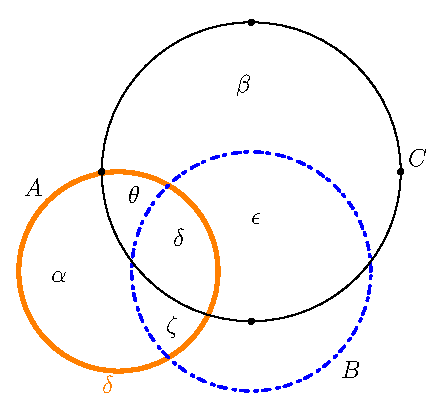
\includegraphics{asy/sets}\centering

\caption{www}
\end{figure}

\begin{defn}
Las \textbf{Variables cuantitativas continuas}, son aquellas variables
que pueden ser representados por los números racionales $\mathbb{Q}$,
``\emph{...que puede tomar cualquier valor en el intervalo considerado}''
\cite[p.~8]{zamora} Por ejemplo la temperatura, el volumen, el peso,
etc. 
\end{defn}

\begin{figure}[!ht]
\centering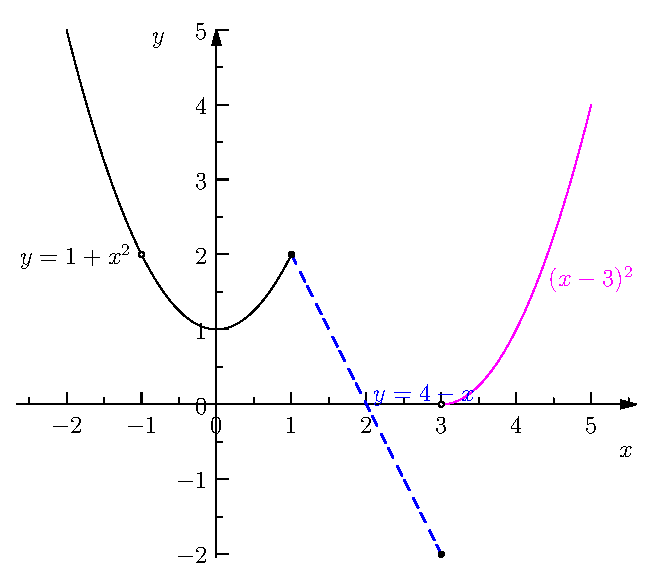
\includegraphics{asy/continua}\caption{Captionwww}
\label{fig:enter-label} 
\end{figure}

www

\section{Organización de datos}

\emph{La distribución de frecuencias}, también llamada \emph{tabla
de frecuencias}, es una herramienta estadística muy útil para organizar
un grupo de datos u observaciones, entre las frecuencias usuales tenemos
a la \textbf{frecuencia absoluta} $f_{i}$ que es el número de veces
que se repite un valor en un conjunto de datos, la suma de todas ellas
es igual al número de datos $\sum_{i=1}^{m}=n$, donde $m\leq n$
es el número de clases. La \textbf{frecuencia acumulada mayor que}
$F_{i}$ es la suma de las frecuencias absolutas desde la primera
hasta la frecuencia $f_{i}$ es decir $F_{i}=\sum_{j=1}^{i}f_{j}=f_{1}+f_{2}+\cdots+f_{i}$
observe que $F_{m}=\sum_{i=1}^{m}f_{i}=n$. La \textbf{frecuencia
acumulada menor que} $F_{i}^{*}$ es la suma de las frecuencias absolutas
desde $f_{i}$ hasta la frecuencia absoluta $f_{m}$ es decir $F_{i}=\sum_{j=i}^{m}f_{j}=f_{i}+f_{i+1}+\cdots+f_{m}$.

La \textbf{frecuencia relativa} $h_{i}=\frac{f_{i}}{n}$, observe
que $\sum_{i=1}^{m}h_{i}=\sum_{i=1}^{m}\frac{f_{i}}{n}=\frac{f_{1}+f_{2}+\cdots+f_{m}}{n}=\frac{n}{n}$,
donde $m$ es el número de clases La \textbf{frecuencia relativa acumulada
menor que} $H_{i}=\frac{F_{i}}{n}$, se tiene que $H_{m}=1$ La \textbf{frecuencia
relativa acumulada mayor que} $H_{i}^{*}=\frac{F_{i}^{*}}{n}$, observe
que $H_{1}^{*}=n$

La \textbf{frecuencia relativa porcentual} $h_{i}\%=100h_{i}$ la
propiedad es que la suma de todas ellas nos genera el $100\%$ es
decir $\sum_{i=1}^{m}h_{i}\%=100\%$, $m$ es el número de clases
La \textbf{frecuencia relativa acumulada menor que porcentual} $H_{i}\%=100H_{i}$,
$H_{m}=100\%$ La \textbf{frecuencia relativa acumulada mayor que
porcentual} $H_{i}^{*}\%=100H_{i}$, $H_{1}^{*}\%=100\%$

\subsection{Datos no agrupados}

Esta distribución de frecuencias se utiliza cuando los datos son cualitativas
nominales u ordinales y cuantitativos discretos solo si estos no tienen
muchas clases, en caso contrario se utilizara la siguiente distribución
de frecuencias para datos agrupados. Aquellos datos que siguen una
jerarquía deben ser ordenados en forma ascendente.

\begin{table}[ht!]
\centering %
\begin{tabular}{|c|c|c|c|c|}
\hline 
$\sum_{1}^{3}f\left(x\right)dx=\lim_{\triangle x\to\infty}f\left(x\right)\triangle x$  & w & w & $w$ & w\tabularnewline
\hline 
\hline 
w  & w & w & w & w\tabularnewline
\hline 
w  & w & w & w & w\tabularnewline
\hline 
w  & w & w & w & w\tabularnewline
\hline 
\end{tabular}\caption{Datos tabulados de una variable cuantitativa discreta}
\label{11} 
\end{table}


\subsection{Datos agrupados \ref{11}}

\begin{figure}
\centering\subfloat[wwwww]{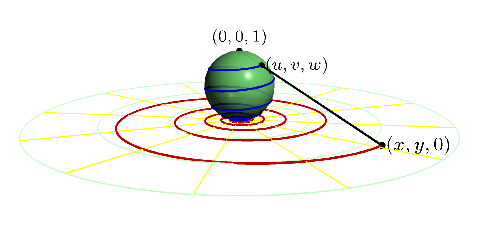
\includegraphics{asy/3dwww}

}\subfloat[www]{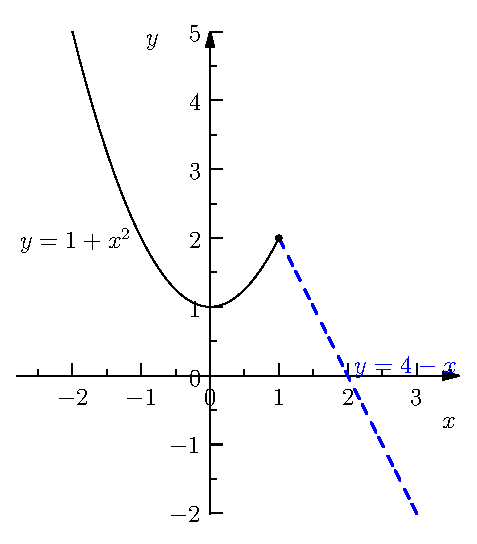
\includegraphics{asy/plane2}

}

\caption{wwwwwwww}
\end{figure}

Esta distribución se usa cuando la variable es cuantitativa continua
o cuando el número de valores distintos de una variable cuantitativa
discreta es demasiado grande (mas de 20). Se halla el número de intervalos
que agruparan a los datos $m$, lo cual esta restringido entre 5 y
20, ``\emph{muchos intervalos pueden complicar los innecesariamente
los cálculos de las medidas descriptivas y pocos intervalos podrían
omitir características importantes de los datos}'' \cite{zamora}.
Determinar el rango $R=x_{max}-x_{min}$, determinar el número de
intervalos por el método de $k=\sqrt{n}$ si $25\leq n\leq100$ o
$k=1+3.3\log n$, $n\geq10$ redondeado al entero inmediato superior.
Determinar la amplitud interválica $c$, dividiendo el rango por el
número de intervalos $c=\frac{R}{k}$ si $c$ no es exacta en el número
de decimales de los datos, entonces $c$ se aproxima por \emph{exceso}
de manera que se cubra todo el rango

Si los datos son enteros $c$, es entero. si los datos tienen un decimal
, $c$ tiene un decimal, etc. Por ejemplo , si los datos tienen do
decimales y si $c=\frac{R}{k}=5.3416$, se elige $c=5.35$ (no 5.34)

Determinar los extremos de los intervalos de la siguiente manera $I_{1}=[x_{min},x_{min}+c[$,
$I_{2}=[x_{min}+c,x_{min}+2c[$, ... $I_{k}=[x_{min}+\cc{k+1}c,x_{min}+\cc{k}c[$.
El ultimo intervalo se cierra por la derecha. Esto se debe a que si
la división $\frac{R}{k}$ es exacta en el número de decimales de
los datos, entonces, $x_{max}=x_{min}+kc$

\begin{table}[ht!]
\centering 
\begin{centering}
wwwwww 
\par\end{centering}
\caption{Datos tabulados de una variable cuantitativa continua}
\label{22} 
\end{table}


\section{Gráficos estadísticos}
\begin{defn}
Sectores circulares son utilizados para representar todas las distribuciones,
``\emph{los datos de cada categoría se representa por un sector circular
cuyo ángulo central es $\alpha_{i}=360^{\circ}h_{i}$}'' \cite{zamora} 
\end{defn}

\begin{figure}
www

\caption{wwwww}
\end{figure}

%Por ejemplo considerando el Cuadro \ref{11} tenemos que $\alpha_1=360^\circ h_1=360^\circ\cdot\STtag{t1}=\FVal{\STtag{t1}*360}^\circ$, $\alpha_2=\FVal{\STtag{t2}*360}^\circ$, $\alpha_3=\FVal{\STtag{t3}*360}^\circ$, $\alpha_4=\FVal{\STtag{t4}*360}^\circ$, $\alpha_5=\FVal{\STtag{t5}*360}^\circ$, $\alpha_6=\FVal{\STtag{t6}*360}^\circ$, $\alpha_7=\FVal{\STtag{t7}*360}^\circ$ y $\alpha_8=\FVal{\STtag{t8}*360}^\circ$. Refiérase a la Figura \ref{44}

\begin{figure}
\subfloat[www]{\centering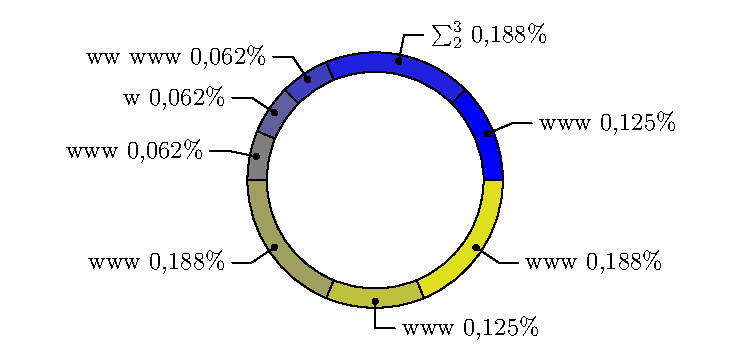
\includegraphics{asy/round}

}\subfloat[www]{\centering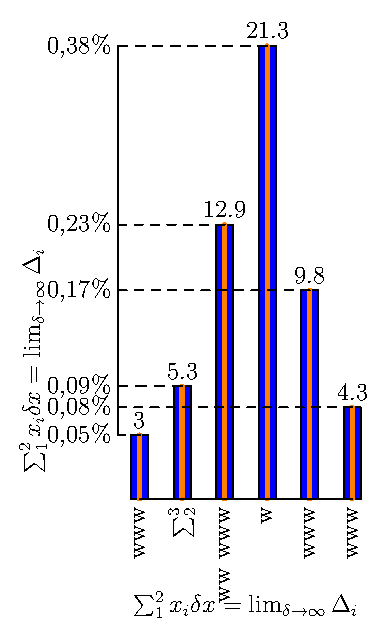
\includegraphics{asy/bar}

}

\caption{www}
\end{figure}

\begin{defn}
Gráfico de barras, este tipo de gráficos son utilizados cuando la
variable es cualitativa ``las barras se dibujan dejando un espacio
entre ellas'' \cite{zamora}, de altura igual a la frecuencia absoluta
o relativa, en caso de ser ordinales, las clases se ordenan de izquierda
a derecha. 
\end{defn}

\begin{defn}
Gráfica de bastón específicamente para variables cuantitativas discretas,``\emph{consiste
en trazar en cada valor distinto de la variable, segmentos de recta
que proporcionen a su frecuencia}'' \cite{zamora}. Por ejemplo se
tiene una representación de uno de estos, para la distribución de
frecuencias del Cuadro \ref{11} en la Figura \ref{44} 
\end{defn}

\begin{defn}
Histograma de frecuencias solo cuando la variable es cuantitativa
continua. \cite{zamora} ``\emph{Es gráfica de barras rectangulares
verticales juntas. La base de cada barrages proporcional a la amplitud
del intervalo, y la altura es proporcional a sus frecuencia (absoluta,
relativa o porcentaje)}''. En base esto se consigue otro gráfico
llamado el \emph{polígono de frecuencias} que consiste en unir los
puntos medios de las bases superiores de las rectángulos que componen
el histogram de frecuencias. Se cierra en amos extremos en las marcas
de clase adyacentes de frecuencia cero 
\end{defn}

\begin{thm}
wwwwwwwww 
\end{thm}


\section{Estadígrafos}

\subsection{Medidas de tendencia central}

\subsubsection{Media}

En el caso de $n$ datos no tabulados se tiene $\overline{x}=\frac{\sum_{i=1}^{n}x_{i}}{n}$
en el caso de $n$ datos tabulados en $m$ clases se tiene $\overline{x}=\frac{\sum_{i=1}^{m}f_{i}x_{i}}{n}$
esto es valido para datos agrupados considerando las $x_{i}$ como
las marcas de clase de cada intervalo es decir $\overline{x}=\frac{\sum_{i=1}^{m}f_{i}m_{i}}{n}$

\subsubsection{Mediana}

Es el datos que ocupa la posición central de los datos ordenadas en
forma creciente. En el caso de datos no tabulados si $n$ es impar
la mediana es el dato de la posición $\frac{n+1}{2}$, $x_{\frac{n+1}{2}}$
en caso contrario si $n$ es par, se interpolan los datos centrales
es decir $Me=\frac{x_{\frac{n}{2}}+x_{\frac{n}{2}+1}}{2}$. En el
caso de datos tabulados se sigue el mismo procedimiento anterior.
En el caso de datos agrupados la mediana es un caso particular del
cuartil $Q_{2}$, el decil $D_{5}$ o el percentil $P_{50}$ es decir
$Me=Q_{2}=D_{5}=P_{10}=L_{i}+\frac{\frac{n}{2}-F_{i-1}}{f_{i}}c$
donde $c$ es la amplitud interválica, $L_{i}$ es el límite inferior
del intervalo donde esta el la posición $\frac{n}{2}$, $f_{i}$ la
frecuencia absoluta correspondiente a este intervalo, $F_{i-1}$ la
frecuencia acumulada anterior a este intervalo.

\subsubsection{Moda}

El es dato o conjunto de datos que mas se repiten. En el caso de datos
tabulados es la clase con mayor frecuencia absoluta. En el caso de
datos agrupados es $Mo=L_{i}+\co{\frac{f_{i}-f_{i-1}}{\cc{f_{i}-f_{i-1}}+\cc{f_{i}-f_{i-1}}}}c$,
donde $c$ es la amplitud interválica, $L_{i}$ límite inferior de
intervalo que contiene a la mayor frecuencia, $f_{i}$ la mayor frecuencia
absoluta, $f_{i-1}$ y $f_{i+1}$ son las frecuencias absolutas adyacentes
a $f_{i}$.

\subsection{Medidas de dispersion}

\subsubsection{Varianza y desviación estándar}

En el caso de datos no tabulados la varianza es $S_{x}^{2}=\frac{\sum_{i=1}^{n}\cc{x_{i}-\overline{x}}^{2}}{n-1}$,
$n$ es el número de datos. En el caso de datos tabulados se tiene
que $S_{x}^{2}=\frac{\sum_{i=1}^{m}f_{i}\cc{x_{i}-\overline{x}}^{2}}{n-1}$
donde $m$ es el número de clases y $x_{i}$ la clase correspondiente.
En el caso de datos agrupados es $S_{x}^{2}=\frac{\sum_{i=1}^{m}f_{i}\cc{x_{i}-\overline{x}}^{2}}{n-1}$
donde $x_{i}$ es la marca de clase de cada uno de los $m$ intervalos.
En todos los casos la desviación estándar es la raíz cuadrada de la
varianza $S_{x}=\sqrt{S_{x}^{2}}$.

\subsubsection{Coeficiente de variacióncd cd}

Este estadígrafo nos dice que tan dispersos están los datos uno de
otros, obedece a siguiente formula $CV=100\frac{S_{x}}{\overline{x}}\%$

\subsection{Medidas de posición}

%referencial textual
Los cuantiles son los estídagrafos para medir la posición entre las
mas importantes se tiene a los cuartiles, los deciles y los percentiles,
las cuales dividen a los datos ordenados en forma ascendente, en cuatro,
diez, cien, partes iguales respectivamente, en el caso de datos no
agrupados se tiene el dato que ocupa en la posición $\frac{\left(n+1\right)j}{N}$.
En el caso de datos agrupados se tiene $C_{j}=L_{i}+c\frac{\frac{jn}{N}-F_{i-1}}{f_{i}}$.
donde $n$ el número de datos $N$ es el número de distribuciones
en que se divide el cuantil, $j$ es el cuantil, $F_{i-1}$ es la
frecuencia acumulada anterior a intervalo que contiene al de la posición
$\frac{jn}{N}$, $f_{i}$ es la frecuencia correspondiente a este
intervalo, $L_{i}$ es el límite inferior de este intervalo y $c$
es la amplitud interválica.

\section{Práctica guiada}

(30 minutos) incluye dos momentos: 
\begin{enumerate}
\item \textbf{Monitoreo:} el profesor supervisa que todos los grupos de
estudiantes elaboren las respectivas tablas de distribución de frecuencias
y los gráficos estadísticos relacionados, y colaboren mutuamente en
el proceso deduciendo ideas principales y secundarais infiriendo otras,
implícitas en el prontuario. 
\item \textbf{Diagnóstico de dificultades en el aprendizaje:} recogidos
la practica grupal en los papelotes y las respectivas respuestas,
el docente determinará el número de estudiantes que evidencian errores
en las respuestas, de ubicarse que hay una cantidad considerable de
alumnos con equivocaciones o no hayan respondido, se realizará un
diagnóstico y discusión sobre las dificultades encontradas y luego
se hará un reforzamiento de aquellos temas no comprendidos.

Preguntas inferenciales: 
\begin{itemize}
\item ¿Que tipo de distribución de frecuencias se de utilizar en cada conjunto
de datos? 
\item Es importante para usted el uso de la tabla de distribución de frecuencias.
¿Por qué? 
\item ¿Por qué es importante los gráficos estadísticos? 
\item ¿Cuáles son las bondades de la técnica exposición--discusión? 
\end{itemize}
\end{enumerate}
\cite{Barnsley}\bibliographystyle{apacann}
\bibliography{www}
 \raggedright
\thispagestyle{empty} 
\end{document}
